
\documentclass[12pt]{article}
\usepackage{fullpage}
\usepackage{graphicx}
\usepackage{array}
\usepackage{subcaption}
\usepackage{caption}
\usepackage{float}
\usepackage{hyperref}
\usepackage[utf8]{inputenc}
\usepackage{setspace}

\title{4982V Senior Design: HUBERT}

\author{
	Hunter Messner\\messn036@umn.edu\\
}
\date{\today}
\setcounter{secnumdepth}{0}
\doublespacing
\begin{document}
	
	\maketitle
	
	\tableofcontents
	
	\listoffigures
	\newpage
	\section{Abstract}
	A new computing paradigm called Hybrid Binary-Unary (HBU) has the potential to further improve computer efficiency by reducing the amount of hardware needed to perform calculations. Though still in the early stages of development, this technique can be applied where low precision and low bit width can be tolerated. HUBERT is an application of this technique that is meant to showcase the practicality and the benefits of adopting HBU in AI applications.
	The goal of the HUBERT project is threefold. First, to implement HBU computation in a practical context to further its development and adoption. Second, to develop a pipeline of technology that can be used to convert an application to HBU. Finally, to increase performance of AI inference on FPGAs, which is specific to the HUBERT application. 
	
	In this project, the I-BERT language AI model is the target of optimization. HUBERT development is not finished, and so the HUBERT project only optimized the GELU function at the time of this paper. This GELU function is used in the inference step of I-BERT. Though there are more potential targets of optimization, difficulty in development limits this project’s data to that collected for GELU. However, the pipeline for HBU development is clearly laid out in this paper and can be used in future projects. The results of HUBERT show how one might identify a target of optimization, how to use HLS techniques to simulate hardware results of an implementation, and how to compare a binary function to a hybrid unary-binary function in the practical example of GELU. The results of an optimized GELU are a good example for Unary improvements. The results of comparison, although limited, show that the HBU implementation uses 4.35\% of the resources of the binary version, a marked improvement.
	
	\section{Introduction}
	The problem: AI models are getting very large and take up lots of computing resources when deployed commercially. The solution: HUBERT, an implementation of an AI where Hybrid-Binary Unary computation is used to optimize said AI for server and commercial use.
	
	Modern natural language processing (NLP) models are large and computation intensive. Since they are used in web apps like autocomplete, search, and translate, NLPs are often deployed in a commercial context. Though often less efficient than GPUs, FPGAs allow engineers to optimize the model and continue improving the performance over time. This also allows the adoption of new technologies that take advantage of FPGA resources on a whim. One such technology that should be adopted is Hybrid Binary-Unary (HBU) computation.
	
	This paradigm has the potential to make functions that meet certain criteria orders of magnitude more efficient. Functions best optimized by HBU are bounded, low-precision functions. In contemporary computing, these are often found in AI/ML models like BERT. An NLP AI like BERT \cite{bert} is often deployed commercially with FPGA accelerators. Since HBU technology can only be deployed on FPGAs so far, this makes BERT a great target for optimization. The HUBERT implementation further improves upon I-BERT \cite{ibert} an integer only version of BERT. When reading this paper, it is important to keep HUBERT and I-BERT straight. I-BERT shall mean the high-level synthesis version of the I-BERT project which originally written in python. HUBERT is functionally the same as I-BERT but is accelerated with HBU functions. Both can be deployed on any FPGA.
	
	HUBERT uses a technology called high-level synthesis (HLS) to compile and generate resource utilization results. This data allows the comparison of HBU to traditional methods (binary). HLS allows developers to deploy programs written in a special flavor of C/C++ to FPGAs, rather than forcing them to rewrite their programs in verilog. Modern HLS compilers allow developers to collect data about accuracy, area usage, and delay. These metrics are used to directly compare I-BERT to HUBERT and quantify the improvements.
	This project is a proof-of-concept implementation. Thus, the data that is collected compares a base version of the code to the optimized version for analysis. This project is not complete; however, results for the GELU sub function have been collected and give a good idea of the results of the entire project. The resource utilization via the Area*Delay metric is gathered through the Intel Quartus HLS compiler whose target is a Cyclone10GX FPGA.
	
	In addition to solving the problem of optimization, and possibly more importantly, HUBERT furthers the adoption of HBU computing by providing a pipeline for developers to use. This is important because development in HLS is not widespread. Making unary more accessible by providing an example project could inspire more research into the subject and its applications. The pipeline detailed by the code of this project covers the development environment, the technologies used, strategies for problem solving, and testing. This code and its wiki are publicly available at \url{https://github.com/DeanKamen/HUBERT}.
	
	\section{Previous work}
	Hybrid Binary-Unary (HBU) is the core of the project and its ultimate motivation. This technology finds a way to minimize the amount of resources needed to compute one input, one output functions by taking advantage of unary logic, which requires a fraction of the logic gates. This method is similar to integer-only math as it takes advantage of quantization to improve performance. When quantizing a function with integer math, one must set bounds on both input and output. Then, one can “scale” the result of integer operations to match the range of numbers that would be represented by floating point \cite{quantizing}. Unary takes this one step further and unpacks integers themselves to be more efficient in hardware \cite{unary}. The downside of this unpacking is that the cost of HBU explodes when trying to represent bit widths above 16. Thus, HBU is only efficient for low bit widths. HBU is “hybrid” because it assumes that most operations will be done in binary. When a unary function is needed, the binary values will be converted to unary, computed, and then converted back to binary. Thus, the best applications for unary are when there exist functions (or a series of functions) that are low precision, quantizable, and expensive to compute. This occurs very often in AI applications in both training and inference. 
	\\
	The description from the paper Routing Magic \cite{unary} is the best way to describe how Unary works.
	\begin{enumerate}
	\item Binary is converted to unary using “thermometer encoders”
	\item A scaling network is used, followed by voting gates to apply a function
	\item All of this is followed by an adder tree to convert unary back to binary
	\end{enumerate}
	An example of this analogy is in Figure \ref{fig:thermometer}, taken from \textit{Hybrid binary-unary hardware accelerator} \cite{hbu}. It demonstrates step two of the process, which is the scaling network. HBU uses a different type of number format, which is not as compact as binary in memory, but does not require as many logic gates to compute results. This number format is called left flushed Unary, where all of the high bits occupy the leftmost bits of a number. In Figure \ref{fig:thermometer}, the inputs are left-flushed unary. For 16 bit width unary, the number 7 is represented as 1111111000000000. Keeping that in mind, the input to output mapping becomes intuitive. If the slope is 1, there is a 1:1 mapping between input and output as shown in Figure \ref{fig:thermometer}. The second part of the figure shows how XOR gates are used to subtract outputs from an arbitrary function so that it does not have to be monotonically increasing.
	
\begin{figure}[h!]
	\begin{subfigure}{.5\textwidth}
		\centering
		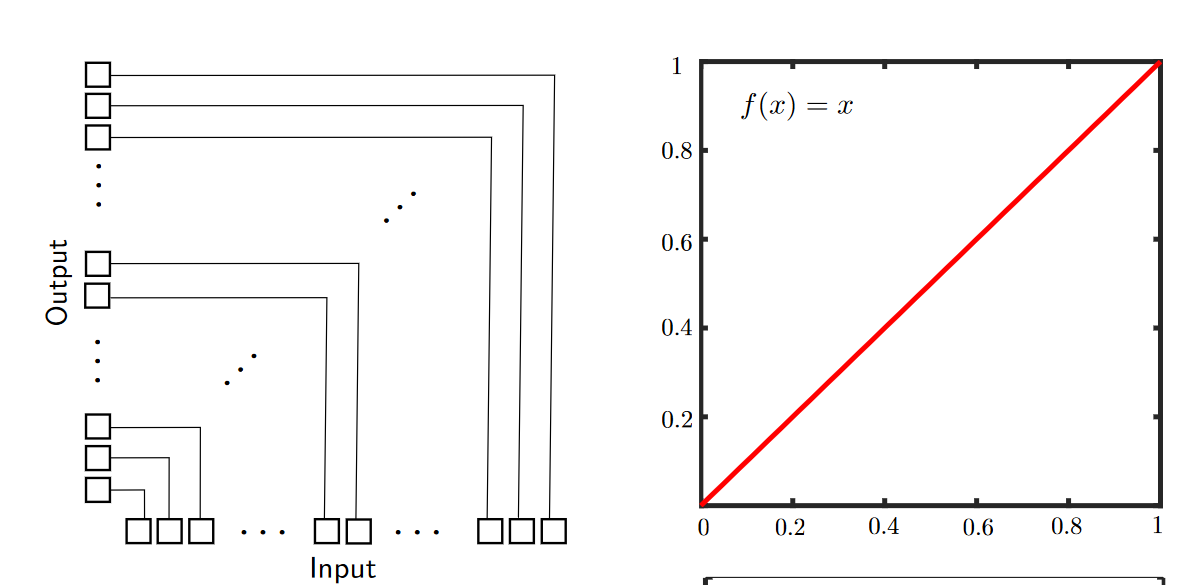
\includegraphics[height=\linewidth]{figures/thermometer1.png}
		\caption{}
	\end{subfigure}%
	\\
	\begin{subfigure}{.5\textwidth}
		\centering
		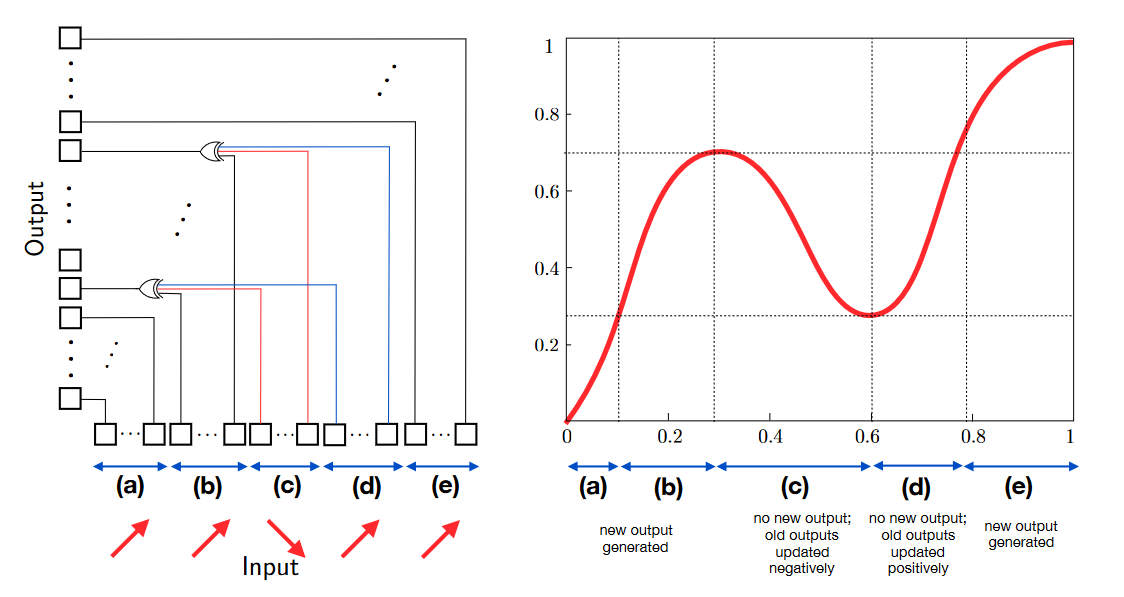
\includegraphics[height=\linewidth]{figures/thermometer2.png}
		\caption{}
	\end{subfigure}%
	\caption{Two examples of Unary functions.}
	\label{fig:thermometer}
\end{figure}
	In Figure \ref{fig:table_prev}, the table compares the logic needed in binary vs the logic needed in HBU for common functions. It also compares the delay. To make a computation faster, the design often needs to take up more area on the FPGA board. Since, in hardware design, there is often a proportional trade off between area and delay, this metric is used to summarize performance. The figure below shows that Unary functions take anywhere from 3\% - 30\% of the Area * Delay product of binary functions! Note that delay is especially low in unary computation, as the analogous nature of HBU allows for completion in a single cycle.
\begin{figure}[h!]
	\centering
	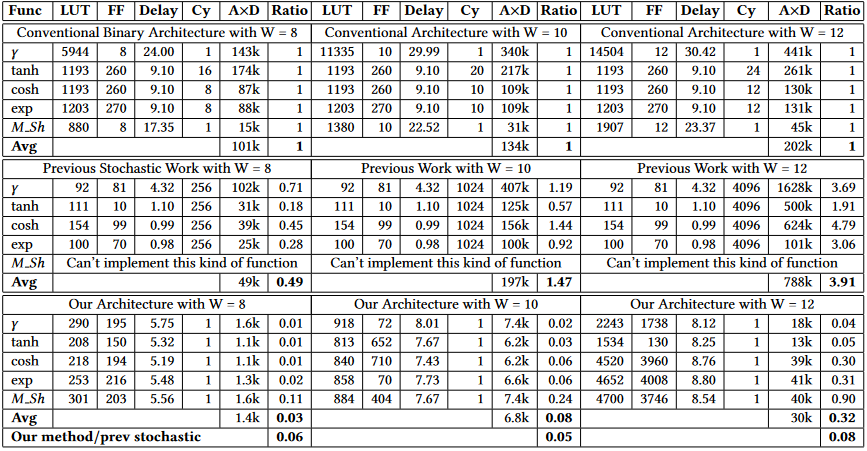
\includegraphics[width=\linewidth]{figures/table_prev.png}
	\caption{FPGA area*delay results from previous work \cite{hbu}.}
	\label{fig:table_prev}
\end{figure}	
	Many of the functions in Figure \ref{fig:table_prev} appear repeatedly in computing. Additionally, when done in batches, many are accelerated by GPU or FPGA accelerators \cite{hbu}. Since AI uses highly parallel techniques and very large batches, AI is a great application for HBU improvements.
	
	One should note that the implementation of HBU computing is limited to the FPGA platform so far. This is because the FPGA is customizable and has many routing resources. It also helps to develop on an FPGA to compare the performance of different architectures. This paper does not provide guidance on how to write an HBU function. HUBERT addresses the FPGA development pipeline and HBU implementation, and it treats functions written in HBU as a prerequisite.
	
	\section{Background}
	\subsection{I-BERT}
	A transformational paper for language processing was published in 2017 and titled \textit{Attention is all you need} \cite{attention}. This paper proposed a way to implement language processing in a way that only uses attention mechanisms. This is relevant as it changed many commercial NLPs from convolutional neural networks to so-called “transformers”. The operations done by transformers can be done in parallel, and are accelerated by custom hardware. This is why commercial deployments of this technology utilize FPGAs. 
\begin{figure}[h!]
	\centering
	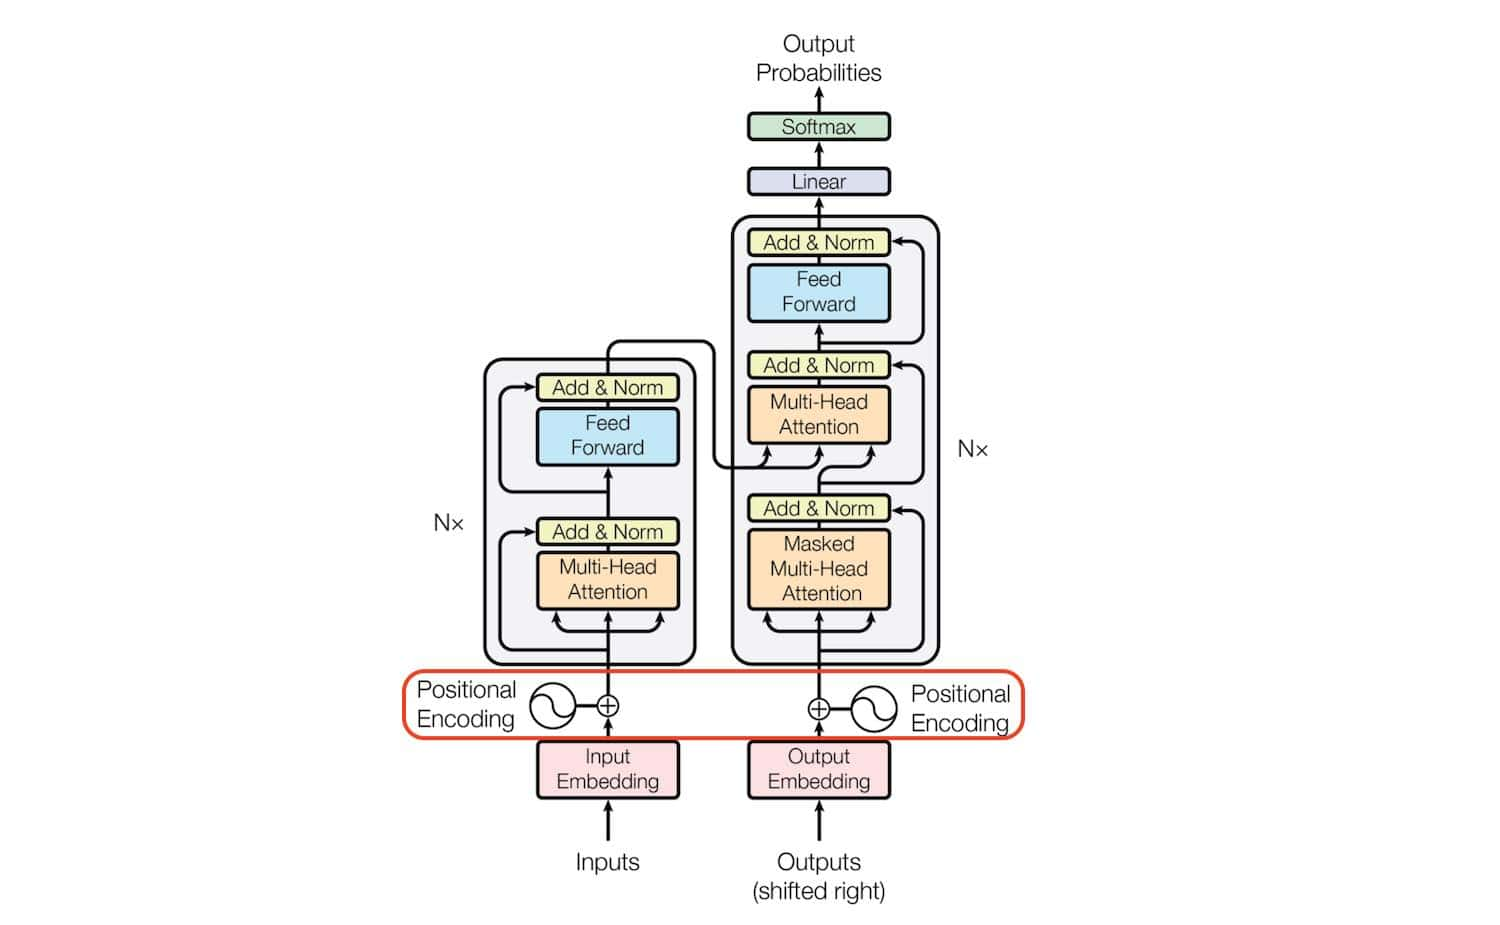
\includegraphics[width=\linewidth]{figures/topology.png}
	\caption{Architecture proposed in Attention is all you need \cite{attention}}
	\label{fig:topology}
\end{figure}	
	
	One such implementation of transformer models is BERT \cite{bert}. BERT is simply a two way language transformer whose pre-training has the purpose of generalizability to various language tasks. The topography of one layer of BERT is shown in Figure \ref{fig:topology}. It details some of the sub functions that are important to all transformer architectures such as Softmax. GELU is notably missing, but was a stage added later as BERT was improved. Each box in the figure represents a mathematical operation that is performed on thousands of weights at once. BERT is typically used to translate between languages, complete sentences, or other NLP tasks. A recent improvement to this model is roBERTa \cite{roberta}. This pre-trained language model is based on BERT but trained more robustly. The inference stage of BERT or roBERTa is compute intensive, and needs the computing power of a data center to perform inference. 
	A project called I-BERT \cite{ibert} aimed to decrease the power consumption and compute time needed for inference by using integer-only math. Integer-only computation can be done faster and on more devices than floating point math. Functions in I-BERT still require a fractional part, however. To solve this, the authors used a method of quantization which uses two integers to represent a floating value. The first is the integer which utilizes its full range, the second is a scaling factor which is used to divide the integer back into the appropriate floating point number. This method only works when the input and output of a function have a known range beforehand. During the training process, this range is learned and the scaling factors are made constants. Thus, after training, I-BERT uses only the integer part to do computation. “With 8-bit quantization, one can reduce the model size by a factor of 4, with negligible accuracy loss. This can be done without needing any data as only the weights are quantized” \cite{quantizing}. This method was proven to be effective in the I-BERT paper. This also proves the assertion that I-BERT is resistant to noise, rounding errors, and accuracy loss, all of which happen in small amounts with the techniques of quantization used. The I-BERT model using 16-bit integer math is a ripe target for improvements using HBU computations.
	The method used to implement HUBERT requires that the python code is translated from python to C++. This is because of the use of HLS to synthesize and compare this project. The I-BERT model is open source and can be found at \url{https://github.com/kssteven418/I-BERT}.
	
	\subsection{HLS}
	The typical development pipeline for FPGAs involves writing verilog, which is a register-level language that requires the developer to control everything that happens each clock cycle. This code is difficult to develop without large amounts of IP (libraries) to build off of.
	High level synthesis (HLS) is a compiler that enables quick prototyping and synthesis of FPGA designs. It does this by compiling C++ code into verilog and organizing a Xilinx/Quartus project to be synthesized using existing tools. The C++ code must follow strict guidelines that pertain to the limitations of FPGAs. This means that common constructs like dynamic memory allocation cannot be used when writing HLS compliant C code. The comparison between regular C code and HLS compliant code is shown in Figure \ref{fig:code}. 
	\begin{figure}[h!]
		\begin{subfigure}{.5\textwidth}
			\centering
			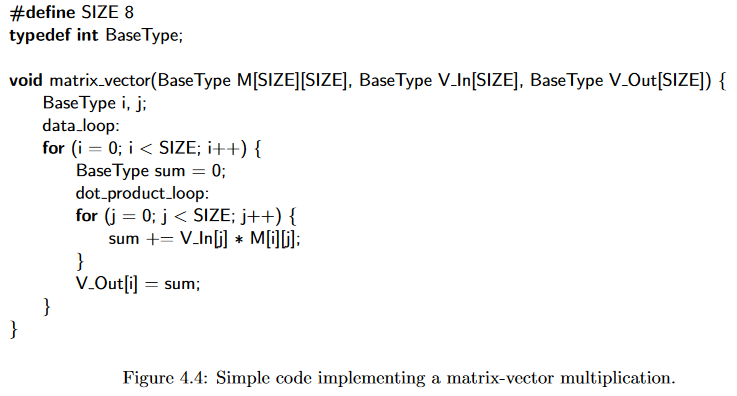
\includegraphics[height=\linewidth]{figures/code1.png}
			\caption{}
		\end{subfigure}%
		\\
		\begin{subfigure}{.5\textwidth}
			\centering
			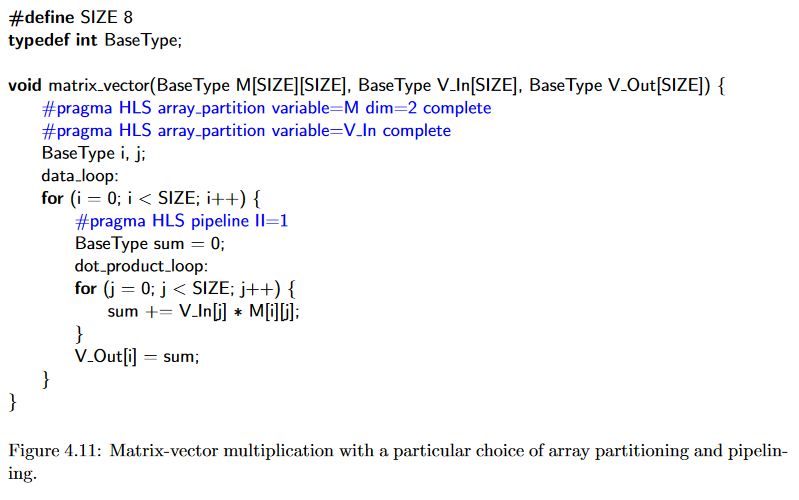
\includegraphics[height=\linewidth]{figures/code2.png}
			\caption{}
		\end{subfigure}%
		\caption{Comparison between C and HLS}
		\label{fig:code}
	\end{figure}
	
	The HUBERT project is currently using the Intel HLS compiler that is included with the Intel Quartus software to test the code. The project, when synthesized, will give a baseline for the Area and Delay needed to deploy the AI model. The goal of this project is to eventually implement all functions that make up one BERT layer. HLS will be used to synthesize both the original and improved project with Unary implemented, since both will be written in C. The difference between each implementation is that HUBERT replaces GELU with its unary equivalent. The Unary functions are written in verilog, but can be easily called by HLS with its RTL integration. HLS generates results about Area and Delay once the project is compiled. This allows for easy comparison in performance metrics. Measuring accuracy can be done with HLS as well, though it is a different process.
	\newpage
	\section{Methodology}
	HUBERT aims to implement I-BERT in C++ in such a way that it can be compiled with HLS. It also aims to replace some one-input, one-output functions with a more efficient HBU equivalent. The HUBERT project is not complete, but the pipeline of development has been created and documented. This is a general pipeline any project can follow. This pipeline assumes that the HBU accelerator module is already developed, and that the project is written in a scripting language.
	
	The first step in this process is to translate the scripting language to C or C++ code. This first translation allows analysis of differences in how compiled code behaves before any other modification. The next step is to make the C code HLS compliant. This step is typically very involved, as most programs utilize dynamic memory allocation. Libraries may have to be rewritten and code refactored. Additionally, the developer must add directives to the HLS compiler indicating where memory dependencies are. The next step is to create a copy of the code that calls the HBU function. If desired, a model of the HBU function can be created in C so that simulations can be run for accuracy. Now that there are two models that share much of the same code base, they can be compared and optimized side by side. The final step is to synthesize and compare the two models. HLS offers many tools and metrics for comparison. Iterating on the final design typically involves the optimization process of HLS development, detailed in the book \cite{textbook}. Figure \ref{fig:flowchart} summarizes this process. 
	
	\begin{figure}[h!]
		\centering
		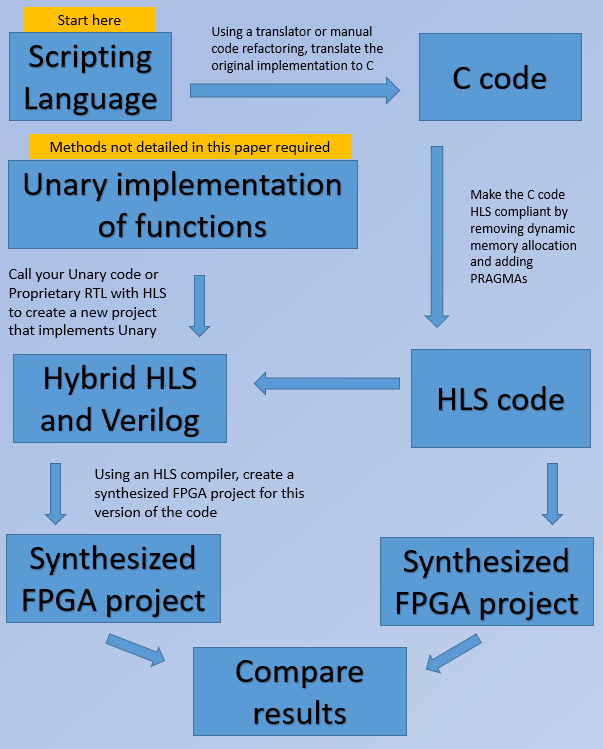
\includegraphics[height=\linewidth]{figures/flow_chart.png}
		\caption{The pipeline for HBU development.}
		\label{fig:flowchart}
	\end{figure}

	So far, in the development of HUBERT, each step in this process has been followed. While the HUBERT project was being developed, so was the development pipeline. This resulted in extraneous development that was not used in the final implementation.
	
	The first step, translating the scripting language to C++, was done via manual code refactoring. The I-BERT code base uses PyTorch, a Machine learning and Tensor library. This had to be re-written in C++. This step requires little technical knowledge.
	
	The second step in the process is making the C++ code HLS compliant. This took the most time in the project. The Tensor operations had to be changed to use no dynamic memory allocation, which was a long process. The difficulty is finding a representation for a Tensor that does not use classes because C++ objects and classes are not fully supported by HLS.
	
	An additional step taken by the HUBERT project is specific to the I-BERT project and does not always need to be done. This step involved making all operations integer operations. This should have been done with the first step, as I-BERT used pseudo integers to simulate integer-only math. In the HUBERT project, delaying this step was a mistake, as it required most of the code to be entirely rewritten. Because of this mistake and time constraints, only the GELU function was rewritten properly. The rest of the pipeline was only completed for the GELU sub-function.
	
	The third step in the process is branching the project and calling the HBU function. This process was difficult in HUBERT as the HBU function was one input, one output but the conventional method was Tensor input and Tensor output. This results in difficulty in optimization and analysis. Additionally, the constants needed to compute GELU are not able to be utilized properly in the HBU function. This resulted in the accuracy metrics generated by HLS being useless. These differences limit the analysis of the results.
	
	The final step in the process is compilation, synthesis, and analysis. HUBERT compilation and synthesis was done with the Intel Quartus suite. The results generated by this service allow the reporting of area, latency, and delay. Accuracy was foregone due to the issues mentioned above. The analysis is limited due to the different implementations of the conventional binary and HBU methods.
	
	As a final note, this process includes little optimization. This means that the results presented in this paper are insufficient for industry decision making. Both approaches need to be greatly optimized  before being compared side by side. Additionally, benefits of HBU cannot be contextualized with just one sub-function. The entire I-BERT AI must be implemented to get realistic results. 
	\newpage
	\section*{Data}
	
	\begin{figure}[h!]
		\centering
		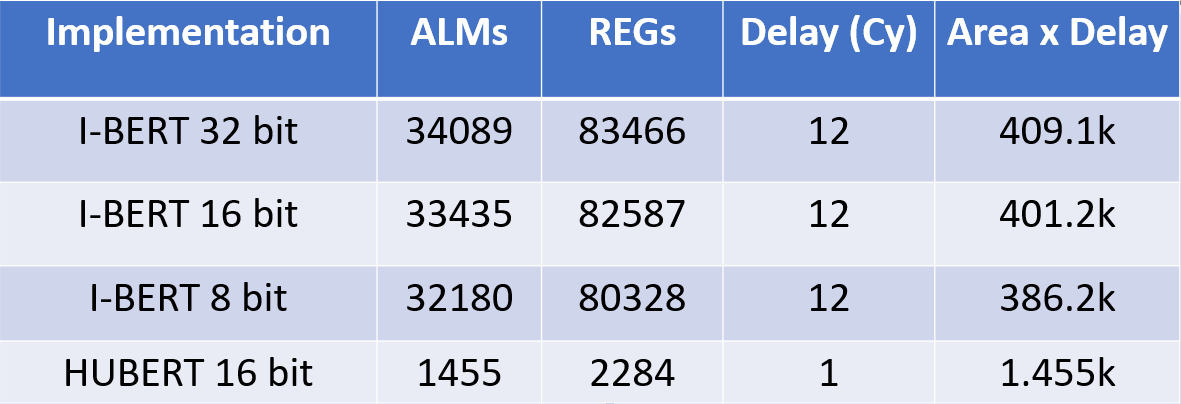
\includegraphics[width=\linewidth]{figures/data.png}
		\caption{Resource comparison between I-BERT and HUBERT.}
		\label{fig:data}
	\end{figure}

	Figure \ref{fig:data} compares I-BERT to HUBERT where I-BERT is the implementation of I-BERT in C and HUBERT is the HBU accelerated version of I-BERT. 16-bit refers to the size of integers used in Tensors.
	\textbf{Area} is the number of ALMs used.
	\textbf{Delay} is the number of cycles between successive outputs.
	
	\begin{figure}[h!]
		\centering
		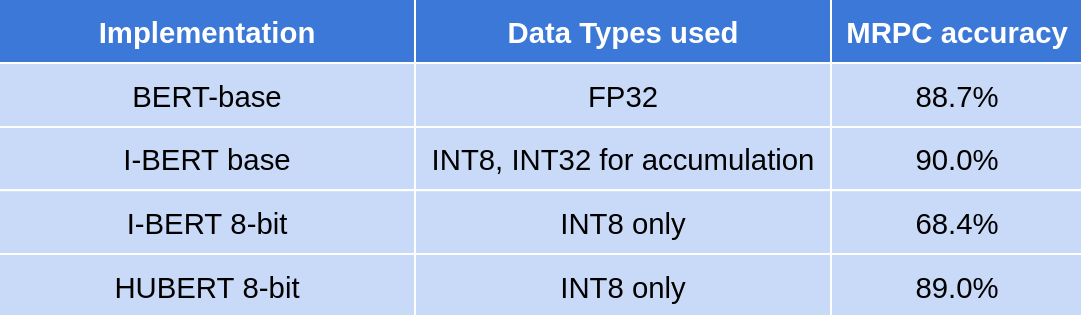
\includegraphics[width=\linewidth]{figures/accuracy.png}
		\caption{Accuracy comparison between I-BERT and HUBERT.}
		\label{fig:accuracy}
	\end{figure}

	Figure \ref{fig:accuracy} compares I-BERT python model accuracy to HUBERT python model accuracy. Note that the I-BERT project \cite{ibert} claimed higher accuracy on BERT base and I-BERT base, but they could not be replicated by the research team. 
	
	\section{Analysis}
	FPGAs have many metrics of analysis. Common ones are efficiency, accuracy, area, delay, and latency. Efficiency is the percent of resources the FPGA program uses on a specific card. Accuracy quantifies the error that comes from a specific hardware implementation of a function. Area is how many resources of a specific type are used. Typically, area is measured in LUTs but in the HUBERT project, it is measured in ALMs. Delay is the number of clock cycles or time in between each output, assuming there is constant input. Latency is the time it takes after giving an input to receive an output. Efficiency is not relevant for research purposes. Accuracy is very relevant to HUBERT, as there is lots of quantization being done to inputs and outputs. However, accuracy data could not be collected for HLS in the time allotted. Area is also important for research purposes, as it better encapsulates how expensive a program is than efficiency. Delay is also important, as it encapsulates the throughput of a system. Latency is sometimes relevant for real time applications, but not in the HUBERT project. 
	
	Programs are made faster through parallelism. By instantiating more math modules on an accelerator, results can be generated in fewer clock cycles. When doing this, Area is increased but delay decreases. Without additional efficiencies, there is an inverse relationship between Area and Delay similar to the inverse relationship between performance and cost. When evaluating this project, decreasing Area or Delay without increasing the other is the goal. This is why the Area * Delay product is the standard way of comparing two FPGA instantiations that give the same output. This metric considers both parallelism and area efficiency.
	
	In HUBERT, this allows comparison between the conventional binary and HBU models. Both produce the same output, but only functionally. They do not use the same architecture or distribution of work. Since each model approaches the problem differently, it is only appropriate to compare performance via the area*delay metric. Comparing area or delay on its own is only in service of computing the area*delay product. Additionally, when comparing accuracy, directly comparing output numbers won't work, but comparing their results on a test will. This is why the python models use the MRPC accuracy as comparison.
	
	The data collected shows a huge difference in Area in Figure \ref{fig:data}. This difference comes from the very specialized way that HBU modules can efficiently implement a one input, one output function. Additionally, HBU gains area improvements by skipping the individual operations of GELU (multiplying, shifting, etc.) and simply implements the analog of this function. The HBU technique clearly worked on GELU and resulted in large performance improvements. The Area of HUBERT is just 4.35\% of that of I-BERT for the same bit width. The data also shows a 12 fold decrease in delay. Unfortunately, this discrepancy is due to a lack of time and experience with FPGA optimization. I-BERT could be optimized to give output within one cycle, and so the analysis will limit its conclusions to the improvement in Area and exclude delay.
	
	The accuracy data in figure \ref{fig:accuracy} shows a general trends of lower accuracy with lower bit widths. This is to be expected. However, when moving from I-BERT base to 8 bit implementations, HUBERT keeps its accuracy higher than I-BERT. Though this data is a testament to the efficacy of HBU quantization, it is not a demonstration of inferiority from I-BERT. I-BERT 8-bit is the HUBERT team's construction of adding an additional quantization layer before GELU to eliminate the use of 32 bit ints. The original GELU model was not designed for this, and its accuracy suffers due to an inability to model GELU accurately with 8-bits. HBU computation works very well with limited quantization width, the reasoning being that it uses the entire quantization range. 
	
	The most proper comparison demonstrating a limited loss of accuracy is between I-BERT base and HUBERT 8-bit. There are a two factors that go into the python accuracy data being so close between the models in Figure \ref{fig:accuracy}. First is the difference of quantization. To utilize the full range of HBU's analog capabilities, the inputs to the HBU function must be the same bit-width as the outputs. Changes were made to HUBERT's python simulation to add an additional quantization layer before GELU so that the 32 bit accumulation INTs could be eliminated. This lets HUBERT maintain high accuracy even when the 32 bit integer are removed. The second factor is that the HBU version of GELU has high fidelity to the original, even in 8 bit. HBU computation can implement GELU correctly as evidenced by a mere 1\% drop in accuracy from I-BERT to HUBERT.
	
	The change in architecture made to HUBERT means that accuracy must be compared through a standardized test. In this case, the MRPC benchmark is the test used. It is noteworthy that this accuracy is high, but also note that this is not HLS accuracy. The results are from a python simulation of the two architectures. This python simulation implements HBU as a lookup table, and there should be no difference from the python simulation to HLS. However, it is possible there may be additional rounding errors introduced in the synthesis step (for both HUBERT and I-BERT) which are not compared in this paper. These differences would arise from the difference between python and C when it comes to rounding integer math.
	
	A 23x better module with small accuracy loss is no small improvement. However there are three caveats to these results.
	The first is that only GELU is implemented. This limits the analysis to that similar to previous work, which is just taking into account the function that needs to be implemented, disregarding other code infrastructure. When the HUBERT project is complete, it will compare an entire layer of I-BERT to that of HUBERT. This gives more information because it is possible that GELU only takes 2\%-3\% of the resources of a whole layer, for example. However, its hard to know the area savings potential until the entire layer is implemented. The optimization could be very impressive if the current bottlenecks have to do with GELU. Analysis of how much savings HUBERT brings to I-BERT on the whole is still an open question. 
	
	The second caveat is that HLS simulation and HLS deployment of the HUBERT module is not implemented. There is a “scaling factor” that is not incorporated into the HBU implementation of GELU. Additionally, a layer of quantization was added to HUBERT, which makes comparison more difficult, as the functionality between a C simulation and python simulation of the two models is not identical. These changes would not have any impact on resource utilization should they be fixed. However, the absence of these simulations does prevent easy HLS accuracy analysis on the system. 
	
	The third caveat is that Accuracy data for HLS is not available. This is because the testing stage involves deploying these programs on an FPGA. Due to time constraints this was not completed. However, the Python simulations are high fidelity and give a good insight into the accuracy penalties of HBU. Additionally, It has been verified that HUBERT is functionally correct through comparing the Python implementation to C. If the rounding done by integer-only math causes accuracy issues, or the deployment to an FPGA causes issues not seen in reporting, this has to be known by the stakeholder. This is why this caveat is being reported in this paper, as the lack of accuracy data for a real deployment may be unacceptable for industry analysis.
	
	\section{Conclusion}
	
	One of the purposes of HUBERT is to implement HBU computation in a practical context to further its development and adoption. The current state of HUBERT is short of this goal. It differentiates itself from previous work by implementing some of the practicalities of being a sub function of an AI. However, these practicalities are limited as the rest of the HUBERT model is not implemented. Another purpose is to show the pipeline of development for HBU acceleration. This goal was met, as the pipeline of development that was discovered over this project is documented well and will work for the rest of the project. The final and most specific goal of HUBERT is to increase performance of AI inference on FPGAs. The data demonstrates that the HUBERT model is more efficient than I-BERT on an FPGA. HUBERT meets this final goal in some capacity.
	
	Bottlenecks in AI optimization are holding back AI development. The most common way of optimizing an AI model is to increase parallelization with operations like matrix multiply. Parallelization can only get one so far when dealing with complex functions like GELU, which take multiple steps to implement. HBU computing can do the whole function in one pass, making it faster. Additionally, the resource savings allow HBU modules to be duplicated across the FPGA so that it is friendly to parallelization. Even though HBU functions can only be applied to one input, one output functions, these are the ones that are most commonly creating bottlenecks in industry. Thus, the savings due to HBU are not trivial. HBU acceleration will likely be considered in commercial contexts.
	
	Overall, the progress of the HUBERT project is promising, and development will continue. The potential benefits of HBU functions are too large to pass up as demonstrated in this paper. HBU technology is slowly breaking ground in the FPGA space, and it may soon be deployed to important applications in industry. This paradigm of acceleration may be key to both scaling up already large networks as well as making AI inference available to the smallest of devices. Both of these improvements could change the AI landscape as we know it.
	
	\bibliographystyle{abbrv}
	\bibliography{Final_bib}
	
\end{document}








